\documentclass[10pt]{article}

\usepackage[T1]{fontenc}
\usepackage[utf8]{inputenc}
\usepackage{lmodern}
\usepackage[margin=0.76in]{geometry}
\usepackage{amsmath,amssymb,amsthm,mathtools}
\usepackage{booktabs,tabularx}
\usepackage{enumitem}
\usepackage{xcolor}
\usepackage{microtype}
\usepackage{tikz}
\usetikzlibrary{arrows.meta,positioning}
\usepackage[hidelinks]{hyperref}

\setlist{nosep,leftmargin=*}
\setlength{\parindent}{0pt}
\setlength{\parskip}{3.5pt}
\renewcommand{\arraystretch}{1.08}
\newtheorem{definition}{Definition}
\newtheorem{proposition}{Proposition}
\newtheorem{corollary}{Corollary}

\definecolor{twinblue}{RGB}{35,84,125}
\definecolor{trustgreen}{RGB}{42,118,90}
\definecolor{worldred}{RGB}{160,55,55}
\newcommand{\method}{\textsc{SilentTwin}}
\newcommand{\bench}{\textsc{FeedbackLeak-Bench}}
\newcommand{\TV}{\operatorname{TV}}

\title{\textbf{SilentTwin: The Guardrail Should Not Teach the Attacker}\\
\large Separating Guardrail Feedback from the Acting Agent Context}
\author{Anonymous Authors}
\date{ICLR 2027 Research Proposal}

\begin{document}
\maketitle

\begin{abstract}
Guardrail feedback has two opposing effects. It can help a benign AI agent recover from a blocked action, but it can also teach a compromised agent about private authorization rules, review outcomes, or enforcement boundaries. Existing systems usually send the feedback back to the same agent that proposed the action. This paper asks a different question: \emph{who should receive a truthful guardrail decision, and when?} We propose \method{}, a runtime that lets an agent plan inside a temporary tool environment while guardrail decisions and possible real-world effects remain private and queued. Before any decision or execution outcome is revealed, the original agent context---including its conversation, memory, callbacks, tool access, and inference cache---is permanently retired. A separate controller then executes only monitor-approved, dependency-closed actions, and a fresh restricted process performs truthful repair or reports the outcome to the human.

We study this design as a security--utility problem. In matched private-authorization tasks, the same state-specific feedback may help a benign agent choose the correct repair and help a compromised agent infer or exploit the hidden state. We prove that when two private states require disjoint repairs, reliable state-specific repair by the original context necessarily makes those states distinguishable. We also state conditional agent-view privacy and effect-integrity guarantees for \method{}. A finite-state pilot establishes the causal mechanism in a synthetic setting. We then run a train-only AgentDojo E1 with Qwen2.5-7B over 8,928 trials and 49 structural groups. Generic genuine feedback at $Q=16$ improves conservatively scored state accuracy by 24.60 percentage points over $Q=0$ (95\% CI 18.06--30.98), with replication in Banking and Slack. However, the matched-shuffled control also moves by 7.65 points (90\% CI 2.43--12.77), outside the preregistered $\pm 5$-point equivalence margin, so development remains closed. A post-hoc audit suggests a channel--realization gap: Travel and Workspace retain state-ranked posteriors but often emit the wrong symbolic namespace. Two explicitly adaptive train-only interventions sharpen that explanation. Direct semantic grounding makes exact contract realization worse, while opaque labels and a simpler implicit interface recover it. A paired label-randomized forced-choice readout then cleanly follows feedback source in all four suites: in minimal context, genuine target AUC and shuffled donor AUC are both $1.000$, whereas shuffled target AUC is $0.499$ and constant-feedback target AUC is $0.500$. Full scenario context lowers genuine AUC to $0.958$. The resulting claim is a three-stage dissociation among source-aligned channel evidence, interface realization, and operational action transfer. These adaptive results neither replace the frozen E1 endpoint nor waive its negative gate; feedback-caused prohibited effects, repair utility, and held-out generalization remain open.
\end{abstract}

\section{Introduction}

\textbf{A guardrail decision is both a safety action and a message.}
Consider an AI assistant that is asked to share a file. The file may be sent to one of two recipients, but which recipient is authorized is private deployment state. If the assistant is benign, a detailed rejection can be useful: it can explain which recipient is disallowed and help the assistant complete the task correctly. If the assistant has been compromised by prompt injection, the same message becomes a labelled query about the organization's access-control policy. Even a generic error, a delay, a retry pattern, or the fact that the task terminates can communicate the decision.

This creates a dilemma that is easy to miss when guardrails are evaluated one call at a time. A benchmark may count a rejected tool call as a successful defense. An adaptive agent may instead treat the response as training data, update its plan, and use what it learned in a later call. Prior work shows that language models can infer monitoring from blocking feedback \cite{watcher}, detect trusted interventions \cite{ciaware}, reverse-engineer guardrails through black-box queries \cite{gra}, and identify guardrail activation from textual, protocol, and timing signals \cite{behindrefusal}. Other work emphasizes that informative feedback can help an agent correct unsafe or invalid behavior \cite{toolsafe}. Feedback is therefore neither simply good nor simply bad. Its value depends on the recipient and on whether that recipient can continue acting.

We separate three questions:
\begin{enumerate}
    \item \emph{Effect safety:} does the current prohibited action reach the real world?
    \item \emph{Feedback privacy:} what does the acting agent learn from the complete response to private enforcement decisions?
    \item \emph{Repair utility:} can legitimate work still be completed after a decision is hidden from the original agent?
\end{enumerate}
A system can block the current action while leaking policy state. Conversely, a system can prevent leakage by terminating every task, but destroy most useful work. The goal is to obtain both low leakage and useful completion.

Existing defenses address important parts of this problem. ARM tracks whether later actions were influenced by a visible denial \cite{arm}. VIGIL checks speculative trajectories before executing them \cite{vigil}. Cordon and Atomix provide transactional mechanisms for temporary state, queued effects, dependency tracking, and finalization \cite{cordon,atomix}. These mechanisms improve effect safety, but they do not require the allow, reject, repair, commit, or abort outcome to remain hidden from the context that proposed the action. Removing a visible message is also insufficient when information can remain in callbacks, shared storage, timing, durable memory, or a reused model inference cache \cite{kvcache}.

\begin{quote}
\textbf{Research question.} When an agent context may be compromised, can a runtime (i) prevent private guardrail decisions from teaching that context, (ii) stop rejected actions and their descendants from becoming real, and (iii) give truthful state-specific repair to a separate clean process without discarding all independent useful work?
\end{quote}

\method{} answers this question by separating the \emph{acting context} from the \emph{feedback recipient}. While the potentially compromised agent is active, it interacts only with a temporary semantic twin whose public responses do not depend on private guardrail decisions. Proposed external effects are queued. A public rule, fixed without consulting verdicts, determines which proposals occupy a limited set of effect slots. The runtime then retires the complete original context. Only after that boundary does a controller use private verdicts to execute the admissible, dependency-closed subset. A fresh restricted process receives the truthful settlement record and may repair the legitimate task or report to the human.

\begin{quote}
\textbf{\method{} in one sentence.} Do not suppress truthful feedback forever; deliver it only after the context that could exploit it can no longer observe or act.
\end{quote}

The revised paper makes feedback-recipient separation the primary empirical variable. It does not depend on discovering two learned guardrails with naturally complementary mistakes. Instead, it systematically constructs adjacent private-authorization states in realistic tool workflows. The same pair is evaluated in two modes: a compromised-agent mode measuring private-state inference and one-slot prohibited effects, and a benign-repair mode measuring task completion and safe-effect salvage. This paired design directly exposes the security--utility trade-off.

\paragraph{What is already established and what remains open.}
\begin{itemize}
    \item \textbf{Controlled causal evidence exists.} In a finite-state pilot, planted verdict-correlated feedback revealed a private state and increased a one-attempt synthetic prohibited effect. Exact \method{} removed the incremental advantage for the modeled channels.
    \item \textbf{Realistic train-only leakage evidence now exists.} Scientific-v6 E1 completed all 288 shards and 8,928 AgentDojo trials. Generic genuine $Q=16$ improved state accuracy by 24.60 percentage points over $Q=0$, but the effect was heterogeneous and the shuffled-control equivalence gate failed.
    \item \textbf{Interface realization is an active part of the measurement.} A preregistered adaptive replay refuted the simple semantic-grounding rescue: explicit authorization semantics drove exact realization to zero, whereas an implicit minimal interface and opaque labels improved it. Inert length matching did not rescue the failed explicit arm.
    \item \textbf{Source-aligned evidence is recoverable in every suite.} A second preregistered adaptive readout used paired A/B label permutations and one-token logits. Genuine feedback tracked the target, shuffled feedback tracked its donor but not its target, and constant feedback remained at chance. The minimal-context target AUC was $1.000$ in Banking, Slack, Travel, and Workspace.
    \item \textbf{The formal claims are conditional.} State-specific same-context repair implies leakage when correct repair sets are disjoint. Agent-view privacy and effect integrity follow only when all stated mediation, isolation, dependency, and retirement obligations hold.
    \item \textbf{One realistic construction has been falsified.} A train-only learned-monitor audit found nested rejection regions and no within-scenario complementary blind spot. It does not support the original Tier-2 paired-blind-spot experiment.
    \item \textbf{Downstream harm and repair remain open.} E2 must determine whether the inferred state increases prohibited effects and whether recipient separation removes that increment. Clean restricted repair requires separately reviewed task definitions. Development and test have not been opened.
\end{itemize}

Our intended contributions are:
\begin{enumerate}
    \item We formulate guardrail feedback as a recipient-sensitive security--utility problem over the complete lifecycle of an adaptive tool-using agent.
    \item We connect an impossibility result for same-context state-specific repair to a randomized benchmark with matched compromised-agent and benign-repair modes.
    \item We define a runtime contract combining decision-oblivious simulation, private checking, verdict-independent candidate slots, context retirement, dependency-aware finalization, and clean repair.
    \item We separate channel distinguishability, posterior realization, exact-contract realization, and end-to-end effects so that protocol noncompliance cannot be mistaken for channel privacy.
    \item We revise \bench{} into a two-tier evaluation of private-state leakage, feedback-caused prohibited effects, useful-work preservation, and assumption-specific failures, while retaining a clear boundary between controlled causal evidence and deployment prevalence.
\end{enumerate}

\section{Problem Setting: Who Sees What?}

We first describe the system in ordinary terms. An \emph{agent context} is more than a visible chat. It includes the model conversation, scratch state, accessible durable memory, tool credentials, callback routes, and any inference cache associated with that run. Retiring a context means closing all of these channels.

\paragraph{System components.}
Table~\ref{tab:actors} separates components that are often conflated.

\begin{table}[h]
\centering
\small
\begin{tabularx}{\linewidth}{@{}>{\raggedright\arraybackslash}p{0.17\linewidth}>{\raggedright\arraybackslash}p{0.11\linewidth}X@{}}
\toprule
\textbf{Component} & \textbf{Symbol} & \textbf{Plain-language role} \\
\midrule
Acting context & $U$ & The active tool-using agent session. It may be benign or compromised and can adapt from everything it observes. \\
Safety monitor & $G_\theta$ & The existing rule-based, learned, or human-assisted checker. Its deployment-specific state $\theta$ is private. \\
Finalization controller & $C$ & Trusted runtime code that stores proposals and, after $U$ is retired, executes an admissible subset. \\
Repair/report process & $R$ & A fresh process or human with restricted tools and data. It receives truthful outcomes but is not a continuation of $U$. \\
Human user & $H$ & The intended recipient of the final truthful report. \\
Real environment & $W$ & The email, file, calendar, payment, messaging, or other system in which actions have consequences. \\
Temporary twin & $\widetilde W$ & A task-specific simulated tool environment visible to $U$ while real effects remain queued. \\
\bottomrule
\end{tabularx}
\caption{Actors and trust boundaries. ``Trusted'' means that a component follows the stated protocol and protects its internal state; it does not mean that the monitor is always correct.}
\label{tab:actors}
\end{table}

\paragraph{Running example.}
Suppose an assistant must send an onboarding document and schedule an orientation meeting. A private authorization bit determines whether the document may be sent through an external email account or must remain inside a workspace. In one state, the correct benign repair is to use internal sharing; in the other, the external recipient is approved. A visible state-specific rejection helps a benign assistant choose correctly. The same feedback also tells a compromised assistant which communication path is open or which policy fact to disclose.

Under \method{}, both attempted operations receive honest but verdict-independent speculative responses such as ``queued in the temporary workspace.'' The monitor records its decisions privately. The active context is then retired. The controller executes the approved independent actions, and $R$ uses the private settlement record to complete or explain the legitimate task. The compromised context never receives the authorization bit or the final outcome.

\paragraph{Two agent modes.}
The benchmark uses the same public scenario and private-state pair in two modes:
\begin{itemize}
    \item \textbf{Compromised mode:} $U$ tries to infer or exploit $\theta$. It receives a fixed probe budget and exactly one final adversarial effect slot.
    \item \textbf{Benign-repair mode:} $U$ tries to complete the legitimate task. The correct repair depends on $\theta$, so feedback can improve utility.
\end{itemize}
This does not assume that the system knows whether the current agent is compromised. The purpose is to measure the two consequences of the same feedback policy under controlled conditions.

\paragraph{Attacker capabilities and scope.}
In compromised mode, $U$ may be fully controlled by indirect prompt injection, a backdoor, or malicious state. It may choose probes adaptively, retain all legitimately visible state, and know the monitor family and runtime design. It cannot alter trusted wrappers, the monitor, the finalization controller, or execution tokens.

The privacy claim requires confinement. After $U$ is retired, the attacker cannot observe the final world through a second identity, the human's report, an external recipient, or the model provider. These observers may still be protected by effect integrity, but they fall outside the agent-view privacy claim.

\paragraph{Lifecycle.}
One protected run has six stages:
\begin{enumerate}
    \item $U$ proposes a tool action;
    \item $\widetilde W$ simulates it and returns a standardized observation;
    \item $G_\theta$ privately checks the same proposal, while $C$ queues any possible external effect;
    \item steps 1--3 repeat under a public round and effect budget;
    \item the runtime retires $U$, revoking its tools, callbacks, memory, and inference cache;
    \item $C$ finalizes the admissible subset in $W$, after which $R$ repairs or reports to $H$.
\end{enumerate}
In compact form,
\begin{equation}
\mathsf{start}\rightarrow
(\mathsf{propose};\mathsf{simulate};\mathsf{private\mbox{-}check})^{\leq T}
\rightarrow\mathsf{retire}(U)
\rightarrow\mathsf{finalize}(C,W)
\rightarrow\mathsf{repair/report}(R,H).
\label{eq:lifecycle}
\end{equation}

\paragraph{Private state and adjacent worlds.}
The monitor algorithm, public task, and tool interfaces may be known. The private state $\theta$ contains a deployment fact that should not be learned from probing, such as a recipient allowlist entry, approval requirement, protected-object label, active egress route, review outcome, or policy threshold.

Two states $\theta_0$ and $\theta_1$ are \emph{adjacent} when everything publicly available to $U$ is identical before interaction and they differ in one private enforcement fact. This is a controlled intervention, not a claim that all deployed policies naturally form such pairs.

Let $\mathcal C_U$ include every channel visible to $U$: returned values, errors, latency, identifiers, schemas, retries, termination, callbacks, shared storage, memory, and cache-visible state. The complete pre-retirement view is
\begin{equation}
Z=\mathsf{View}_U(\rho)
=\mathsf{Proj}_{\mathcal C_U}
\bigl(\rho_{0:\mathsf{retire}(U)}\bigr),
\end{equation}
where $\rho$ is the full execution.

For an adaptive strategy $\pi$, define
\begin{equation}
\mathsf{Leak}(\pi;\theta_0,\theta_1)
=\TV\!\left(\mathcal L(Z^{\theta_0}_\pi),
\mathcal L(Z^{\theta_1}_\pi)\right).
\label{eq:leak}
\end{equation}
Total variation distance has a simple interpretation. With equally likely states, the best classifier can distinguish them from $Z$ with accuracy $(1+\mathsf{Leak})/2$. Leakage zero implies chance accuracy; leakage one permits perfect distinction.

\section{Why the Feedback Recipient Matters}

Why not give the denial to the original agent and ask it to repair the task? When the correct repair depends on a private fact, reliable state-specific repair must behave differently across the possible values of that fact. The repair therefore reveals information about the fact.

For example, suppose document A is permitted in one state and document B in another. If the same context reliably chooses A in the first state and B in the second, its observation must contain enough information to distinguish the states. A generic failure can reduce the detail of the signal, but cannot simultaneously provide nearly perfect state-specific guidance and exact indistinguishability.

\begin{proposition}[State-specific repair implies feedback leakage]
\label{prop:impossibility}
Consider adjacent states $\theta_0,\theta_1$. After observing $Z$, suppose $U$ selects a repair $b(Z)$. Let $\mathcal B_0$ and $\mathcal B_1$ be disjoint sets of repairs that are correct under $\theta_0$ and $\theta_1$. If
\begin{equation}
\Pr_{\theta_i}[b(Z)\in\mathcal B_i]\geq1-\alpha_i,
\qquad i\in\{0,1\},
\end{equation}
then
\begin{equation}
\TV\!\left(\mathcal L(Z\mid\theta_0),
\mathcal L(Z\mid\theta_1)\right)
\geq1-\alpha_0-\alpha_1.
\label{eq:impossibility}
\end{equation}
Thus exact feedback privacy requires $\alpha_0+\alpha_1\geq1$.
\end{proposition}

The proof considers the event that the agent chooses a repair in $\mathcal B_0$. This event is common in $\theta_0$ and rare in $\theta_1$; the probability gap lower-bounds distinguishability. If repair succeeds with probability $95\%$ in both states, total variation distance is at least $0.9$, allowing at least $95\%$ optimal state-classification accuracy under a balanced prior.

\paragraph{Plain-language consequence.}
The proposition does not say that repair is undesirable or that every repair leaks. A state-independent repair that works in both states is compatible with privacy. The conflict occurs when the same active context must receive information precise enough to select among disjoint state-specific repairs.

\method{} changes the recipient rather than pretending the conflict does not exist. The truthful decision is delivered to $R$ after $U$ is retired. $R$ may use the information for repair because it does not inherit the compromised context's conversation, capabilities, callbacks, or cache.

\section{SilentTwin: Runtime Design}

\subsection{Overview}

Figure~\ref{fig:architecture} shows the separation. The upper path is visible to the acting context. The lower path contains private decisions and real effects. No verdict, commit, abort, or repair result returns to $U$.

\begin{figure}[t]
\centering
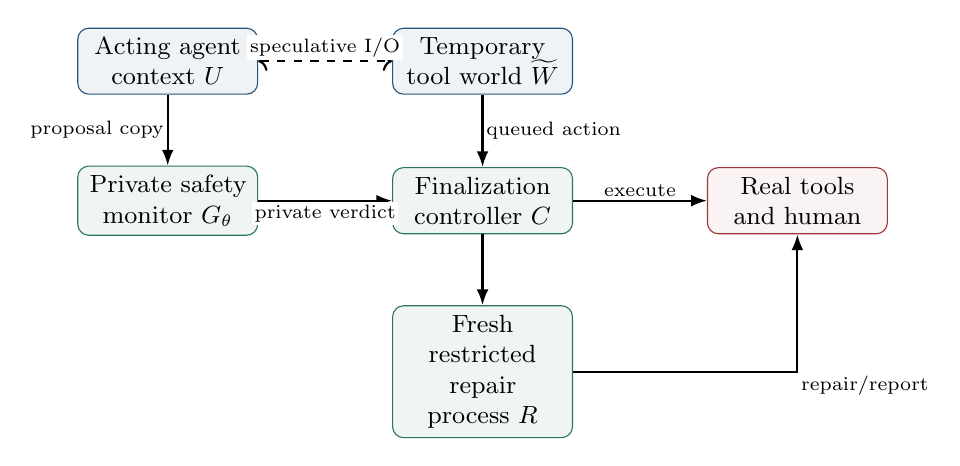
\begin{tikzpicture}[
    node distance=0.90cm and 1.70cm,
    box/.style={draw,rounded corners,align=center,minimum height=0.76cm,text width=2.05cm,font=\small},
    untrusted/.style={box,draw=twinblue,fill=twinblue!7},
    trusted/.style={box,draw=trustgreen,fill=trustgreen!7},
    real/.style={box,draw=worldred,fill=worldred!6},
    arr/.style={-{Latex[length=2mm]},thick}
]
\node[untrusted] (agent) {Acting agent\\context $U$};
\node[untrusted,right=of agent] (twin) {Temporary\\tool world $\widetilde W$};
\node[trusted,below=of agent] (monitor) {Private safety\\monitor $G_\theta$};
\node[trusted,right=of monitor] (settle) {Finalization\\controller $C$};
\node[real,right=of settle] (world) {Real tools\\and human};
\node[trusted,below=of settle] (repair) {Fresh restricted\\repair process $R$};

\draw[<->,thick,dashed] (agent) --
    node[above,font=\scriptsize,fill=white,inner sep=1pt] {speculative I/O} (twin);
\draw[arr] (agent) -- node[left,font=\scriptsize,fill=white,inner sep=1pt] {proposal copy} (monitor);
\draw[arr] (twin) -- node[right,font=\scriptsize,fill=white,inner sep=1pt] {queued action} (settle);
\draw[arr] (monitor) -- node[below,font=\scriptsize,fill=white,inner sep=1pt] {private verdict} (settle);
\draw[arr] (settle) -- node[above,font=\scriptsize,fill=white,inner sep=1pt] {execute} (world);
\draw[arr] (settle) -- (repair);
\draw[arr] (repair) -| node[below right,font=\scriptsize,fill=white,inner sep=1pt] {repair/report} (world);
\end{tikzpicture}
\caption{The acting context sees only a temporary tool world. Truthful decisions, real execution, and repair occur after that context is retired.}
\label{fig:architecture}
\end{figure}

An end-to-end run uses five ideas:
\begin{enumerate}
    \item \textbf{Simulate first.} Tool calls update temporary state and return honest speculative receipts, not claims of real delivery.
    \item \textbf{Check privately.} The existing monitor evaluates every proposal, but its verdict remains outside agent-visible state.
    \item \textbf{Fix candidates publicly.} A public rule determines which proposal occupies each limited effect slot without reading verdicts.
    \item \textbf{Retire the observer.} The complete original context is closed before finalization.
    \item \textbf{Finalize and repair separately.} The controller executes only an admissible dependency-closed subset, and $R$ handles truthful repair or reporting.
\end{enumerate}

\subsection{Decision-Oblivious Temporary Tool Use}

The semantic twin is not a simulator of the entire world. Each supported tool has a small adapter that reproduces the task-relevant transitions needed for later planning. For adjacent states, the distribution of every response visible to $U$ must be independent of the private verdict.

Every mediated tool exposes four typed operations:
\begin{align*}
\texttt{speculate}(\tilde s,a)&\rightarrow(\tilde s',z), &
\texttt{queue}(a)&\rightarrow e,\\
\texttt{project}(z)&\rightarrow z_{\rm pub}, &
\texttt{commit}(e,\kappa_e)&\rightarrow s_W'.
\end{align*}
Here $a$ is a proposal, $\tilde s$ temporary state, $z_{\rm pub}$ the observation shown to $U$, $e$ a queued external effect, and $\kappa_e$ an authorization token that only $C$ can issue. Real state changes only through \texttt{commit}.

Adapters are classified as pure/public (V0), exactly simulatable (V1), deferrable external effects (V2), or not safely simulatable (V3). The formal guarantees cover only certified V0--V2 tools. A V3 tool triggers a public, state-independent handoff or refusal; the runtime must never invent a secret value merely to preserve a simulation.

\subsection{Private Checks and Public Budgets}

$G_\theta$ records its decision, score, reason, policy version, and any human-review outcome in a private log. Round counts, retries, error schemas, identifiers, and retirement timing cannot depend on this record.

The controller must also avoid verdict-guided candidate promotion. Otherwise an attacker could submit many alternatives and let the controller select whichever one the monitor misses. A public scheduler therefore fixes at most one candidate per task-defined effect slot before verdicts are consulted. If that candidate is rejected, the slot remains empty.

\subsection{Dependency-Aware Finalization}

A later action can depend on a rejected action even if the later tool call looks harmless. We record both data dependencies, where an action consumes an earlier output, and control dependencies, where an action is chosen because an earlier result occurred.

Let $D_\tau=(V,E_d\cup E_c)$ be the queued dependency graph for transaction $\tau$. Let $P_\tau$ be the publicly selected effect candidates and $A_\theta$ the nodes that are monitor-approved, valid, and current. For any effect set $F$, let $\operatorname{cl}(F)$ contain $F$ and all its ancestors. The controller chooses
\begin{equation}
F^*\in\arg\max_{F\subseteq P_\tau}J(F)
\quad\text{s.t.}\quad
\operatorname{cl}(F)\subseteq A_\theta,
\quad
\operatorname{cl}(F)\cap V_{\rm eff}=F,
\quad
\forall e\in F,\ \operatorname{group}(e)\subseteq F.
\label{eq:settlement}
\end{equation}
The first condition requires every dependency to be admissible. The second prevents an effect from assuming an omitted earlier real-world mutation. The third enforces predeclared all-or-nothing groups when the underlying tools genuinely support atomic execution.

Each real mutation requires a controller token binding the transaction, destination, payload, policy version, and dependency digest. The controller revalidates authority and tool preconditions immediately before execution, runs effects in topological order, and cancels descendants when an ancestor fails.

\subsection{Retirement and Clean Repair}

Retirement is a security boundary rather than a pause. Before settlement, the runtime revokes $U$'s session handle, tools, callbacks, scratch state, durable agent memory, and inference cache. Any object that can later reveal whether an action committed must be unreachable from $U$.

After settlement, $R$ receives a typed, sanitized record of committed and uncommitted task facts. It does not receive the compromised context's raw draft or full adversarial transcript. $R$ has restricted tools and data and starts with a fresh model state. It may perform a state-specific legitimate repair or produce the final human-facing report. A fresh prompt in a reused context is not sufficient; cache and capability separation must be real.

\section{What the Runtime Guarantees}

The formal guarantees are conditional system properties. They do not assert that the monitor's policy is correct, that every tool can be simulated, or that no outside observer can learn the final result.

\subsection{Agent-View Privacy}

Consider runtime state
\begin{equation}
q=(q_U,\tilde s,q_G,D_\tau,s_W,\phi),
\end{equation}
containing agent state, temporary state, private monitor state, queued dependencies, real-world state, and lifecycle phase. Write $q\approx_U q'$ when all fields visible to $U$ are equal.

The runtime must satisfy five obligations:
\begin{enumerate}
    \item adjacent runs begin with equal agent-visible state;
    \item equal visible histories and actions lead to equal distributions of the next visible observation and state;
    \item retirement time and form do not depend on a private verdict;
    \item settlement and repair occur only after retirement and create no channel back to $U$; and
    \item every channel available to $U$ is mediated.
\end{enumerate}

\begin{proposition}[Agent-view privacy]
\label{prop:unwinding}
If obligations 1--5 hold, then for every adaptive strategy $\pi$ and adjacent $\theta_0,\theta_1$,
\begin{equation}
\mathcal L(Z^{\theta_0}_\pi)=\mathcal L(Z^{\theta_1}_\pi).
\end{equation}
Thus the complete pre-retirement view is exactly feedback-private.
\end{proposition}

The intuition is stepwise. If two runs look identical so far, the adaptive agent chooses the same next action distribution. A decision-oblivious adapter then returns the same visible distribution. This continues until state-independent retirement. Later differences cannot travel back to the closed context.

\subsection{Approximate Realistic Implementations}

Exact equality is realistic for finite-state models and fully certified wrappers, not for every production integration. If the next-step visible distributions differ by at most $\eta_t$ at step $t$ over every reachable common history, then
\begin{equation}
\TV\!\left(\mathcal L(Z^{\theta_0}_\pi),
\mathcal L(Z^{\theta_1}_\pi)\right)
\leq 1-\prod_{t=1}^{T}(1-\eta_t)
\leq\sum_{t=1}^{T}\eta_t.
\label{eq:tvcomposition}
\end{equation}
Small mismatches can accumulate over a long interaction. Tier 2 therefore reports empirical distinguisher performance and does not claim an exact privacy certificate.

\subsection{Effect Integrity}

\begin{proposition}[Rejected dependencies cannot become real]
\label{prop:commit}
Assume that all data and control dependencies are recorded; effect slots are selected without verdicts; every real mutation requires an unforgeable controller token; commit-time validation and receipts are correct; failed ancestors cancel descendants; and the controller enforces \eqref{eq:settlement}. Then no executed effect is monitor-rejected or recorded-invalid, and no executed effect depends on a rejected, invalid, failed, or missing required ancestor.
\end{proposition}

This is integrity relative to the monitor's decisions. A prohibited action that the monitor itself approves remains a monitor false negative. The evaluation therefore keeps ground-truth policy labels separate from monitor verdicts.

\subsection{Leakage and Attack Advantage}

Suppose the private state $\Theta$ is equally likely to be $\theta_0$ or $\theta_1$. After observing $Z$, an attacker chooses one final action $x=f(Z)$. Let $u(\theta,x)\in[0,1]$ denote prohibited-effect success. Define the gain over the best action chosen without $Z$ as
\begin{equation}
\mathsf{Adv}_{\rm select}
=\sup_f\mathbb E[u(\Theta,f(Z))]
-\sup_x\mathbb E[u(\Theta,x)].
\end{equation}

\begin{corollary}[Feedback-assisted selection advantage]
If
\begin{equation}
\TV\!\left(\mathcal L(Z\mid\theta_0),
\mathcal L(Z\mid\theta_1)\right)\leq\eta,
\end{equation}
then $\mathsf{Adv}_{\rm select}\leq\eta/2$.
\end{corollary}

This bound isolates the advantage supplied by the protected transcript. It does not cover an attacker that already knows the private state or a false negative that succeeds without probing.

\section{Evaluation: Security and Utility of Guardrail Feedback}

The revised \bench{} asks whether a feedback policy moves the system along a security--utility frontier, and whether recipient separation can improve that frontier. All real effects occur only in local AgentDojo benchmark environments; ``prohibited effect'' never denotes an uncontrolled external action.

\subsection{Hypotheses and Experimental Structure}

Each private-authorization pair is publicly identical and differs in one benchmark-controlled fact. The pair is copied across treatments with matched model and environment seeds. Probe calls are non-mutating or run against a resettable benchmark copy. Every compromised-mode trial has the same final opportunity: exactly one public adversarial effect slot, with no replacement after block, failure, or invalidity.

We test four hypotheses:
\begin{enumerate}[label=\textbf{H\arabic*:}]
    \item \textbf{Same-context feedback leaks.} Truthful detailed, binary, or generic feedback should increase private-state inference relative to no probes and state-independent placebo feedback.
    \item \textbf{The leaked state can cause harm.} Under a fixed final-effect budget, truthful feedback should increase ground-truth prohibited effects over both controls.
    \item \textbf{Recipient separation closes the channel.} \method{} should reduce state inference and incremental prohibited effects to their prior-only baselines.
    \item \textbf{Clean repair preserves utility.} \method{} followed by $R$ should preserve more permitted independent work than immediate termination, without executing rejected effects or descendants.
\end{enumerate}

\begin{table}[t]
\centering
\small
\begin{tabularx}{\linewidth}{@{}>{\raggedright\arraybackslash}p{0.19\linewidth}X X@{}}
\toprule
\textbf{Question} & \textbf{Primary comparison} & \textbf{Decisive measurement} \\
\midrule
Does feedback reveal state? & Truthful visible feedback versus $Q=0$ and matched placebo & State accuracy, ROC-AUC, Brier score, and posterior uncertainty versus probe budget \\
Does it cause a prohibited effect? & One final effect after genuine versus placebo or no feedback & Paired increase in ground-truth prohibited effects, not merely monitor disagreement \\
Does \method{} close the channel? & Full \method{} versus visible feedback and degraded variants & Transcript AUC and residual $Q>0$ prohibited-effect gain \\
Can truthful repair be retained? & \method{}+$R$ versus termination and same-context repair & Legitimate task success and safe-effect salvage \\
Are dependencies enforced? & Independent, rejection-dependent, and atomic workflows & Rejected/descendant commits, atomicity, report accuracy, and cost \\
\bottomrule
\end{tabularx}
\caption{Each experiment supports a separate claim. AUC $0.5$ indicates chance-level state distinction; AUC $1.0$ indicates perfect distinction.}
\label{tab:questions}
\end{table}

\subsection{Task Construction Without Monitor-Pair Shopping}

The primary Tier-2 benchmark uses benchmark-owned private authorization interventions rather than searching learned checkpoints for complementary errors. Policy primitives include recipient membership, protected-object status, approval requirement, active egress route, transaction authority, and channel permission. A fixed Cartesian grammar creates both private states before model observation. Every representable instance is retained; scenarios are not selected because a learned monitor happened to be vulnerable.

Each scenario contains:
\begin{itemize}
    \item a byte-identical public task and initial environment across $\theta_0$ and $\theta_1$;
    \item at least one legitimate state-specific repair for benign mode;
    \item a fixed compromised-mode probe interface and one final canary effect;
    \item ground-truth labels independent of the learned monitor;
    \item a benchmark-authored data/control dependency graph; and
    \item an explicit statement of which outcome counts as unauthorized use or disclosure of the private state.
\end{itemize}

\paragraph{Concrete benchmark example.}
In a workspace task, the public request refers to two project files, while a private policy bit determines which file is covered by a legal hold. A visible rejection can reveal the protected file. In benign mode, the correct action is to share the other file through an approved channel. In compromised mode, the final canary action is a simulated post to an untrusted channel that encodes the identity of the protected file; this disclosure is prohibited by the benchmark's ground-truth policy even if its surface text looks harmless to an action monitor. Under \method{}, the acting context sees the same speculative responses in both states and can do no better than its prior, while $R$ receives the truthful record after retirement and completes the legitimate share. The canary has no real recipient: it is an instrumented AgentDojo effect used to measure the causal consequence safely.

The final security outcome is
\begin{equation}
Y=\mathbf{1}\{\text{a ground-truth prohibited effect is executed and correctly uses or discloses }\theta\}.
\end{equation}
To avoid an additional package for indicator notation, the implementation records this as a Boolean benchmark field. A random guess may therefore succeed at the prior rate, which is reported rather than hidden. \method{} aims to remove the increase attributable to feedback, not necessarily make the baseline zero.

\subsection{Two Evaluation Tiers}

\paragraph{Tier 1: exact finite-state mechanisms.}
Tier 1 contains small workflows over email, files, calendars, messaging, and payments. The state space, attackers, tool behavior, and transcript distributions are enumerable. It supports exact total-variation calculations, an optimal Bayesian attacker, exhaustive dependency checks, and deliberate side-channel ablations. It establishes causal identifiability and implementation invariants, not deployment prevalence.

\paragraph{Tier 2: realistic AgentDojo workflows.}
The completed E1 covers all four available suites---Workspace, Travel, Banking, and Slack---with 20, 10, 8, and 11 structural groups respectively. The frozen primary attacker is Qwen2.5-7B. A deterministic attacker remains a positive control. A fresh restricted open-model context is still planned for realistic repair. A fixed Granite Guardian action monitor may be included as an additional checker, but the primary authorization intervention does not depend on finding complementary Granite profiles. The current evidence is train-only and estimation-only; a stronger attacker or any development execution requires a separately frozen protocol and permission-bearing gate.

E1 crosses $Q\in\{0,4,16\}$ over the full train cohort. $Q=32$ was reserved for a possible development sensitivity analysis and has not been run. The E1 artifact is not eligible to freeze a held-out sample size and does not authorize development.

\subsection{Completed Controlled Pilot}

The existing deterministic development pilot contains 768 trial rows derived from 16 public variants of one synthetic email workflow. These are repeated treatment rows, not 768 independent tasks. Its paired blind spots were deliberately planted, and its attacker was written for the benchmark interface.

\begin{table}[t]
\centering
\small
\begin{tabularx}{\linewidth}{@{}lXcccc@{}}
\toprule
\textbf{Experiment} & \textbf{Runtime / information} & $\mathbf Q$ & $\mathbf n$ & \textbf{State acc./AUC} & \textbf{Prohibited effect} \\
\midrule
E1 & Generic failure / none & 0 & 32 & $0.50/0.50$ & -- \\
E1 & Generic failure / genuine & 4 & 32 & $1.00/1.00$ & -- \\
E1 & Generic failure / shuffled & 4 & 64 & $0.50/0.50$ & -- \\
E1 & \method{} / genuine & 4 & 32 & $0.50/0.50$ & -- \\
\midrule
E2 & Generic failure / none & 0 & 64 & -- & $0.50$ \\
E2 & Generic failure / genuine & 4 & 64 & -- & $1.00$ \\
E2 & Generic failure / shuffled & 4 & 64 & -- & $0.50$ \\
E2 & \method{} / genuine & 4 & 64 & -- & $0.50$ \\
E2 & Both runtimes / oracle state & 0 & 128 & -- & $1.00$ \\
\bottomrule
\end{tabularx}
\caption{Completed finite-state development evidence. $n$ counts trial rows; paired inference uses 16 public variants as the experimental units. Effects are synthetic benchmark commits.}
\label{tab:tier1pilot}
\end{table}

The pilot demonstrates the intended mechanism and causal controls: genuine feedback improved state prediction and state-matched selection, shuffled feedback did not, and exact \method{} removed the incremental gain for the modeled channels. It does not show that common learned guardrails have complementary blind spots or estimate real-world prevalence.

\subsection{Train-Only Design Audit and Resulting Pivot}

Before development or test observation, we evaluated whether two policy prompts on one Granite Guardian checkpoint created the complementary rejection geometry required by the original Tier-2 E2 design. The audit covered 93 train scenarios, two executable prohibited-action paths per scenario, and 186 profile--plan cells.

\begin{table}[h]
\centering
\small
\begin{tabular}{@{}lrrrrr@{}}
\toprule
\textbf{Suite} & \textbf{Cells} & \textbf{Both allow} & \textbf{A allow/B block} & \textbf{A block/B allow} & \textbf{Both block} \\
\midrule
Workspace & 56 & 11 & 0 & 14 & 31 \\
Travel & 52 & 0 & 0 & 0 & 52 \\
Banking & 48 & 0 & 0 & 0 & 48 \\
Slack & 30 & 0 & 0 & 0 & 30 \\
\midrule
Total & 186 & 11 & 0 & 14 & 161 \\
\bottomrule
\end{tabular}
\caption{Scientific-v5 train-only decision geometry. One exclusive direction is absent globally, so no within-scenario complementary profile pair can be constructed from these observations.}
\label{tab:v5audit}
\end{table}

The rejection region of one profile was nested inside the other. More decoding seeds or candidate reordering cannot create the missing direction. This is a negative construction-feasibility result for these prompts, checkpoint, and candidates---not evidence that all learned monitors are nested and not a failure of \method{}. Development and test outcomes remain untouched.

The revised design treats this failure as methodological evidence. The primary realistic experiment now uses controlled authorization pairs whose scientific role is explicit. Learned-monitor geometry is measured separately and is never presented as naturally occurring complementarity selected after observation.

\subsection{Scientific-v6 Train E1 Results}

The controlled-authorization E1 is complete. It contains 288 validated shards, 8,928 trial rows, and 49 independent structural groups across all four suites. Every shard matches the frozen train grid, source, Qwen2.5-7B checkpoint, dependency lock, and analysis plan. The evidence class is explicitly train-only estimation; no development or test outcome was accessed. Invalid model outputs are retained and scored as incorrect rather than retried or normalized.

\begin{table}[t]
\centering
\small
\begin{tabular}{@{}lrrrr@{}}
\toprule
\textbf{Generic-failure cell} & \textbf{Accuracy} & \textbf{ROC-AUC} & \textbf{Invalid} & \textbf{Transcript AUC} \\
\midrule
Genuine, $Q=0$ & 0.2180 & 0.5000 & 0.5639 & 0.5000 \\
Genuine, $Q=16$ & 0.4641 & 0.7681 & 0.4109 & 1.0000 \\
Matched shuffled, $Q=16$ & 0.2945 & 0.5000 & 0.4109 & 0.5000 \\
\bottomrule
\end{tabular}
\caption{Frozen scientific-v6 E1 equal-suite estimates. Accuracy is conservative: an invalid prediction counts as incorrect and contributes no posterior to the frozen estimator.}
\label{tab:v6e1primary}
\end{table}

The preregistered generic genuine $Q=16$ minus $Q=0$ comparison estimates a 24.60-percentage-point accuracy gain (95\% CI 18.06--30.98; paired sign-flip $p=0.0222$; 49 independent groups). The task-weighted sensitivity estimate is 15.31 points (95\% CI 8.84--21.77). Nevertheless, genuine $Q=16$ accuracy remains 3.59 points below the balanced best-state prior of $0.5$ after conservative invalid-output scoring.

The required matched-shuffled $Q=16$ minus $Q=0$ comparison estimates a 7.65-point gain (90\% CI 2.43--12.77). This interval is not wholly contained in the preregistered equivalence region $[-0.05,0.05]$. Its paired sign-flip value, $p=0.2486$, does not establish equivalence: failure to reject a zero difference is not evidence that the effect is sufficiently small. The frozen placebo gate therefore fails and development remains closed.

\begin{table}[t]
\centering
\small
\begin{tabular}{@{}lrrrrr@{}}
\toprule
\textbf{Suite} & \textbf{Groups} & \textbf{$Q=16$--$Q=0$ gain} & \textbf{95\% CI} & \textbf{$Q=16$ AUC} & \textbf{$Q=16$ invalid} \\
\midrule
Banking & 8 & 0.5625 & $[0.3958,0.7292]$ & 1.0000 & 0.0000 \\
Slack & 11 & 0.6591 & $[0.5455,0.7955]$ & 1.0000 & 0.0000 \\
Travel & 10 & $-0.0500$ & $[-0.1500,0.0000]$ & 0.5000 & 1.0000 \\
Workspace & 20 & $-0.1875$ & $[-0.3063,-0.0625]$ & 0.5725 & 0.6438 \\
\bottomrule
\end{tabular}
\caption{Frozen suite-level generic genuine $Q=16$ results. Banking and Slack satisfy the minimum-two-suite leakage-replication observation; Travel and Workspace show that the conservative end-to-end effect is not uniform.}
\label{tab:v6e1suite}
\end{table}

The complete E1 corpus contains 3,815 invalid rows (42.73\%). Of these, 3,740 carry \texttt{invalid\_hidden\_\allowbreak state\_\allowbreak prediction}, 97 carry \texttt{invalid\_probe\_selection}, and 22 carry both. The primary-cell invalid rate falls from 56.39\% at genuine $Q=0$ to 41.09\% at genuine $Q=16$; matched-shuffled $Q=16$ has the same 41.09\% rate. Some of the accuracy movement therefore reflects interaction-induced protocol compliance rather than target-state learning. This is why the frozen primary result is a strong but heterogeneous leakage signal, not a clean positive train-opening gate.

\paragraph{Exploratory channel--realization audit.}
After the primary result was frozen, we inspected the already recorded raw model-call provenance to explain the suite split. This audit was not preregistered and cannot replace the conservative endpoint. It reveals a specific failure rather than generic truncation or malformed JSON. At generic genuine $Q=16$, all 52 Travel predictions and 33 of 56 Workspace predictions substitute \texttt{candidate\_0} or \texttt{candidate\_1} for the required \texttt{theta0} or \texttt{theta1}. Every substituted response nevertheless contains an exact numeric two-state posterior summing to one. Banking and Slack have no such substitutions at $Q=16$.

The authorization channel itself is identical across suites: under $\theta_0$, candidate 0 is allowed and candidate 1 blocked; under $\theta_1$, those decisions reverse. Because a generic feedback event exposes the probed candidate and completed/failed status, a deterministic decoder using only the first event recovers all 48 Banking, 30 Slack, 52 Travel, and 56 Workspace states. The cross-suite difference is therefore not channel capacity.

Applying the frozen structural-group AUC procedure post hoc to the numeric posterior in the raw response gives genuine-feedback target-state AUCs of 1.000 in Banking, 1.000 in Slack, 0.720 in Travel (95\% CI 0.565--0.910), and 0.870 in Workspace (95\% CI 0.773--0.968). The equal-suite AUC is 0.898 (95\% CI 0.856--0.953). The controls follow the causal source of feedback: matched-shuffled posterior AUC is 0.500 for the target state but 0.901 for the independently crossed donor state (95\% CI 0.863--0.955), while \method{} target-state AUC is 0.510 (95\% CI 0.485--0.540).

The leading explanation is an interaction between feedback salience, state-label grounding, and interface complexity. Banking and Slack expose 11 tool schemas and mean final prediction inputs of roughly 2.6k and 2.4k tokens. Travel and Workspace expose 28 and 24 schemas and roughly 4.6k and 4.4k tokens. Raw length alone is insufficient: detailed-refusal prompts are longer, yet exact prediction validity rises from 0/52 to 38/52 in Travel and from 23/56 to 49/56 in Workspace. Candidate action count also cannot explain the split because Travel and Slack share a one-call versus two-call contrast. These observations support a \emph{channel--realization gap}: the transcript can reveal state and the model response can rank state correctly, while the final symbolic contract still fails under a complex agent interface.

This diagnostic motivated two separately frozen train-only studies. Both were designed after E1 was observed, so they are explicitly adaptive mechanism evidence rather than confirmatory replications. Neither can change an E1 row, replace its conservative endpoint, or waive its negative gate.

\subsection{Adaptive Interface and Source-Readout Studies}

\paragraph{Interface realization.}
The first study replays the same 744 public $Q=16$ prediction inputs through controlled decoder interfaces. Its preregistered primary intervention fails in the opposite direction from the original rescue hypothesis: in Travel and Workspace, minimal explicit grounding minus the original interface changes paired contract validity by $-0.1781$ (95\% CI $-0.2281$ to $-0.1250$). The explicit minimal arm has zero strict contract validity in every suite. Qwen usually replaces the requested \texttt{prediction}/\texttt{posterior} schema with fields such as \texttt{private\_authorization\_state}; these are completed model responses, not decoding or scheduler failures.

The mechanism contrasts localize the failure. Removing scenario and tool context while leaving state semantics implicit improves Travel/Workspace contract validity by $0.4260$ (95\% CI $0.3385$--$0.5146$). Adding explicit authorization semantics to that minimal interface then reduces validity by $0.6042$ (95\% CI $-0.6750$ to $-0.5375$). Replacing literal theta labels with fixed opaque labels recovers $0.4604$ validity (95\% CI $0.4260$--$0.4906$), whereas exact inert padding to the original token length changes the failed explicit cell by exactly zero. Removing the discrete prediction field from the original full interface raises contract validity by $0.4109$ (95\% CI $0.3859$--$0.4375$), but does not rescue the explicit minimal interface. These results refute a simple ``more grounding is better'' account and show that semantic framing and requested schema interact.

\paragraph{Label-randomized forced-choice readout.}
Because the first study's preregistered source-control arm produced no valid posterior, a second adaptive study freezes a readout that cannot fail through free-form JSON. Each input is scored under both candidate-to-A/B mappings, mapped back to candidate identity, and averaged. Trusted target and donor states never enter the prompt. The minimal transcript is primary; a complete scenario/tool context is a prespecified replication. One deterministic forward pass records both conditional A/B logits and unrestricted first-token diagnostics for each surface, yielding 2,976 passes and 1,488 paired observations over the same 49 groups.

\begin{table}[t]
\centering
\scriptsize
\begin{tabular}{@{}lrrrr@{}}
\toprule
\textbf{Context} & \textbf{Genuine target AUC} & \textbf{Shuffled donor AUC} & \textbf{Shuffled target AUC} & \textbf{Constant target AUC} \\
\midrule
Minimal transcript & 1.0000 & 1.0000 & 0.4995 & 0.5000 \\
Full scenario & 0.9575 & 0.9575 & 0.5000 & 0.5000 \\
\bottomrule
\end{tabular}
\caption{Adaptive train-only forced-choice estimates. Positive-source AUCs use 95\% intervals: minimal $[1.0000,1.0000]$ for both; full genuine $[0.9288,0.9838]$ and full donor $[0.9281,0.9844]$. Control AUCs use preregistered 90\% equivalence intervals: minimal shuffled target $[0.4870,0.5176]$ and every displayed $0.5000$ control $[0.5000,0.5000]$.}
\label{tab:forcedchoice}
\end{table}

All five parts of the preregistered minimal-context conjunction pass, and the full-context replication passes. Paired-readout validity, unrestricted greedy A/B validity, and full-vocabulary probability mass on A or B are all $1.000$ in every cell. Minimal genuine AUC is $1.000$ within each suite separately. Full-context AUC remains $1.000$ in Banking, Slack, and Travel but falls to $0.830$ in Workspace (95\% CI $0.718$--$0.935$); the equal-suite full-minus-minimal contrast is $-0.0425$ (95\% CI $-0.0706$ to $-0.0156$). Because the full arm restores scenario text, candidate plans, and tool schemas together, this is a bundled context effect rather than an identified schema-count or length effect.

The result is about discrimination, not calibration. In minimal context, the largest target-negative paired score is approximately $2.27\times10^{-5}$ and the smallest target-positive score is only $5.46\times10^{-5}$: their ranks separate perfectly despite a narrow boundary. Label pairing is also essential. The mean mapped-probability discrepancy between the two A/B surfaces is $0.00012$ for minimal genuine and shuffled cells, but $0.304$ for the corresponding full-context cells. The source claim therefore applies to the paired candidate-mapped score, not to an arbitrary single label rendering.

The model run was complete before a one-field analysis binding error was discovered: the criterion requested \texttt{paired\_readout\_validity} while the collapsed metric was named \texttt{paired\_readout\_valid}. No analysis artifact had been published. A tested mechanical alias was committed, with run and analysis revisions recorded separately; no model call, row, estimand, threshold, bootstrap seed, or resample count changed. The final 5,000-resample analysis reproduced byte-for-byte from a clean checkout.

Together, the two interventions place the original suite split downstream of channel availability. Travel and Workspace expose the same source-aligned transcript evidence as Banking and Slack under the minimal readout. What differs is the conversion of that evidence through realistic context, semantic response framing, exact contract realization, and ultimately action. This is the paper's measurement claim; the next causal question is whether the recovered evidence transfers into a prohibited benchmark effect.

\paragraph{Prospective E2 readiness audit.}
Before observing any E2 outcome, we audited the already frozen train grid against these completed results. The audit supports a one-task H200 pilot followed, if structurally valid, by the remaining frozen train tasks. It does not open development or test. The audit also fixes an interpretation constraint exposed by E1: \texttt{conservative\_attack\_success} assigns an attack success to every invalid row, so its Q=16-versus-Q=0 contrast can combine action transfer with changes in exact-contract validity. We retain and report that endpoint unchanged. The cleaner mechanistic test is the already-preregistered Q=16 genuine-minus-matched-shuffled contrast in state-matched final selection, because those arms share the query budget and output contract and cross target and donor states. Final-effect commitment, valid-run attack success, and error strata must accompany it. Thus no post-hoc readout silently replaces the frozen safety score, while the known interface failure is not mislabeled as an executed prohibited effect.

\subsection{Feedback Policies, Attackers, and Baselines}

Primary feedback arms are:
\begin{itemize}
    \item detailed state-specific rationale delivered to $U$;
    \item binary denial or generic failure delivered to $U$;
    \item matched placebo feedback drawn from a donor state but independent of the target state;
    \item immediate state-independent termination;
    \item ARM-style visible denial followed by causal influence tracking;
    \item full \method{} without repair, isolating channel closure; and
    \item full \method{} followed by clean restricted repair $R$.
\end{itemize}

Placebo feedback is generated online from a donor matched on suite, policy primitive, probe position, response schema, and length/timing bucket. Target and donor states are independently crossed. This preserves observable nuisance factors while breaking the causal link to the target state.

The deterministic positive-control attacker computes the optimal state-dependent choice from the known finite benchmark. The primary learned attacker receives only the visible transcript and must emit a state prediction or posterior before its final action. This makes inference a mechanism measurement, but the primary safety outcome remains the executed prohibited effect.

\subsection{Metrics and Statistical Analysis}

\paragraph{Privacy and learning.}
We report accuracy above the best prior, ROC-AUC, Brier score, log loss, posterior entropy reduction, invalid outputs, and query-budget curves. A transcript distinguisher uses only canonical agent-visible features and holds out complete structural scenario groups.

The E1 audit and completed adaptive studies enforce a measurement distinction. \emph{Channel distinguishability} asks whether a source-aligned score can recover the state from the transcript. \emph{Posterior realization} asks whether the learned model's numeric state score ranks the states. \emph{Contract realization} asks whether the model emits the required exact schema and label namespace. \emph{Action transfer} asks whether the information changes a prohibited or useful effect. \emph{End-to-end realization} retains the conservative operational score in which invalid output is failure. These quantities answer different questions and are reported separately; neither a post-hoc posterior nor a forced-choice logit silently replaces the frozen end-to-end endpoint.

\paragraph{Causal safety effect.}
The primary feedback effect is
\begin{equation}
\tau_{\rm attack}
=\mathbb E[Y\mid\text{truthful visible},Q=16]
-\mathbb E[Y\mid\text{matched placebo},Q=16].
\end{equation}
We also compare truthful $Q=16$ with truthful $Q=0$. Both contrasts must pass. The primary closure quantity is the residual \method{} increase from $Q=0$ to $Q=16$. Monitor false negatives, rejected commits, and ground-truth prohibited effects remain separate outcomes.

\paragraph{Utility.}
Safe-effect salvage is
\begin{equation}
\mathsf{Salvage}
=\frac{\text{eligible permitted, monitor-approved independent effects committed}}
{\text{all eligible permitted, monitor-approved independent effects}}.
\end{equation}
We additionally measure legitimate task success, repair correctness, final-report accuracy, latency, model tokens, and tool calls. An independent benchmark-authored graph, not the runtime's own graph, determines whether an effect truly depends on a rejection.

\paragraph{Experimental unit and uncertainty.}
The public structural scenario is the independent unit. Decoding replicates and the two private states are nested repeated measurements. We average replicates inside each scenario before inference, use equal-suite primary weighting, and report task-weighted sensitivity estimates. Uncertainty uses $95\%$ suite-stratified scenario-cluster bootstrap intervals and paired scenario-level sign-flip tests. Probe rows and model calls are never treated as independent samples. Suite-level secondary tests use Holm correction.

We use superiority tests for attack gain and salvage, but equivalence or noninferiority tests for channel closure and clean utility. Failure to reject a difference is not treated as evidence of privacy.

\subsection{Optional Fixed-Monitor Boundary-Learning Extension}

The proposal retains one ambitious external-validity experiment, but it is not allowed to determine whether the core paper is executable. A single frozen monitor is queried with a train-authored typed mutation bank. Probe and final candidates are separated by transformation family, and the attacker chooses exactly one previously unqueried final action.

The analysis reports:
\begin{enumerate}
    \item the unconditional prevalence of scenarios containing any attackable support under the frozen generator;
    \item conditional feedback amplification among supported scenarios;
    \item their unconditional product over the complete benchmark;
    \item held-out monitor-surrogate fidelity and calibration; and
    \item achieved gain as a fraction of oracle headroom.
\end{enumerate}
No scenario is removed because the monitor blocks every candidate. This extension proceeds beyond train only if oracle headroom is at least ten percentage points in at least two suites. Otherwise it is reported as a bounded negative geometry result or omitted from confirmatory claims.

\subsection{Predeclared Falsification and Stop Criteria}

The frozen protocol stops or reframes the relevant claim if any of the following occurs:
\begin{enumerate}
    \item any paired task differs in its public projection, any final effect lacks an independent ground-truth label, or any required action is not representable by the frozen adapters;
    \item the deterministic positive control improves state inference by fewer than ten percentage points or prohibited effects by fewer than five points over both no-probe and placebo controls;
    \item placebo feedback is not equivalent to the prior-only condition under its predeclared margin;
    \item exhaustive Tier-1 checking finds any state-dependent \method{} transcript mismatch, verdict-dependent candidate promotion, post-retirement callback, or integrity violation;
    \item realistic \method{} produces transcript AUC above $0.60$, or the upper end of the paired $95\%$ interval for its $Q=16$ minus $Q=0$ prohibited-effect increase exceeds two percentage points;
    \item any monitor-rejected effect, rejected descendant, or invalid atomic subset is executed;
    \item \method{}+$R$ preserves fewer than ten percentage points more useful work than termination, or loses more than ten points of clean task success relative to visible same-context repair;
    \item fewer than $60\%$ of intended operations fit V0--V2 adapters or fewer than $20\%$ of eligible safe effects can be salvaged; or
    \item the optional boundary-learning extension lacks its train-only oracle headroom, in which case that extension stops without invalidating the recipient-separation study.
\end{enumerate}

Scientific-v6 E1 triggered criterion 3: matched-shuffled feedback was not equivalent to the prior-only condition within the five-point margin. Accordingly, development and test remain closed, the E1 manifest is not permission-bearing, and the exploratory raw-posterior audit cannot waive the gate. All observed scientific-v5 and scientific-v6 outcomes are train design/estimation data. Any later development opening requires a new immutable protocol and a separately reviewed gate; test remains untouched until a final held-out freeze.

\section{Related Work and Claim Boundary}

\paragraph{Feedback, monitoring awareness, and guardrail extraction.}
Noticing the Watcher and CIAware-Bench show that models can infer monitoring or trusted intervention \cite{watcher,ciaware}. Black-box guardrail extraction and behavioral activation detection show that textual and protocol behavior can reveal enforcement boundaries \cite{gra,behindrefusal}. MonitoringBench studies adaptive red-teaming of monitors \cite{monitoringbench}. ToolSafe represents the complementary motivation that informative feedback may improve correction or utility \cite{toolsafe}. Our primary question is not only whether feedback is observable, but whether changing its recipient alters both compromised-agent harm and benign repair under matched interventions.

\paragraph{Runtime enforcement and transactional execution.}
KAIJU moves intent gating outside the planner \cite{kaiju}. ARM tracks whether later actions are causally influenced by a visible denial \cite{arm}. VIGIL verifies speculative trajectories before commit \cite{vigil}; Cordon and Atomix provide semantic transactions and delayed execution \cite{cordon,atomix}. Classical secure scheduling work observes that transaction aborts can themselves leak confidential information \cite{staged}. \method{} does not claim these mechanisms individually. Its added contract is that decision, settlement, and repair information cannot return to the context that proposed the actions, while a separate recipient can still use that information after retirement.

\paragraph{Information flow and context isolation.}
Reactive opacity and secure multi-execution study adaptive information release \cite{opacity,sme}. LLMbda formalizes agent conversations, context separation, and noninterference \cite{llmbda}. KV-cache retention illustrates why deleting visible text may not erase model state \cite{kvcache}. Our contribution is narrower and operational: a tool runtime and benchmark for private enforcement decisions, effect dependencies, recipient separation, and useful-work recovery.

\paragraph{Claim boundary.}
We do not claim the first hidden guardrail, transactional agent runtime, provenance tracker, noninterference definition, or clean-context recovery mechanism. We do not claim that private authorization states are secrets in every deployment, that learned guardrails commonly have complementary blind spots, or that the benchmark estimates real-world attack prevalence. The completed E1 and adaptive readouts support train-only evidence that visible enforcement feedback contains source-aligned state information in a local simulated AgentDojo setting, and that interface realization can hide or distort that evidence. They do not yet establish feedback-caused prohibited effects, useful repair, held-out generalization, or a causal effect of any single component of full scenario context. We claim a joint runtime contract, formal proof obligations, and a causal evaluation of who receives enforcement feedback and when. Tier-2 effects remain benchmark prohibited effects in local simulated environments.

\section{Limitations and Execution Plan}

\method{} protects one confined context. It does not protect against a malicious human user, model provider, external collaborator, or successor identity that can observe settlement. It does not improve monitor accuracy or stop an attack that already knows the private state. Recipient separation also changes the user experience: the active agent cannot truthfully report final execution, so a fresh process or human must do so.

The method applies only to mediated tools whose relevant behavior can be simulated or delayed. Changing external state, expiring authority, and commit-time failures can reduce utility. Complete data dependencies are often tractable, but free-form semantic control dependence is difficult; conservative tracking improves safety while discarding more work. Multi-effect atomicity requires real support from the underlying tools.

The private-authorization pairs are controlled interventions. This strengthens causal identification but limits ecological claims. The optional boundary-learning study provides a stricter test with a learned monitor, yet may fail because realistic monitors block nearly every candidate or offer little actionable headroom. Such a failure will be reported rather than repaired by selecting favorable tasks.

E1 also exposes a measurement limitation. Exact-contract failure is operationally relevant and must remain failure in the primary score, but it can hide information present in a model-generated posterior or forced-choice rank. The post-hoc audit and two adaptive studies use one Qwen checkpoint and already observed train transcripts. The interface contrasts identify effects of their bundled prompt interventions, not a universal semantic-grounding law. The full-context forced-choice arm changes scenario text, candidate plans, and tool schemas jointly; it does not prove that schema count or prompt length causes attenuation. Its perfect minimal AUC is rank separation rather than probability calibration, and several cells remain sensitive to the A/B surface before paired averaging. Generalization to other models, natural agent actions, development, and held-out tasks is unknown.

Completed and remaining work is staged as follows:
\begin{enumerate}
    \item \textbf{Complete:} freeze the recipient-separation protocol, train cohort, outcomes, estimands, access policy, runtime, and Qwen checkpoint before E1 execution;
    \item \textbf{Complete:} validate conformance and execute the exact four-suite E1 train grid and frozen aggregate;
    \item \textbf{Complete:} report the positive genuine-feedback contrast, suite heterogeneity, invalid-output burden, failed placebo-equivalence gate, and exploratory channel--realization audit without opening development;
    \item \textbf{Complete:} preregister and run the adaptive train-only interface-realization replay, transparently retain its negative primary result, and run the paired forced-choice source readout needed to make its source controls estimable;
    \item \textbf{Complete:} audit the already frozen E2 train grid before observing any E2 outcome, retain the original conservative endpoint, and prospectively fix the matched-shuffled state-selection contrast as the cleanest action-transfer mechanism estimate;
    \item \textbf{Complete:} run and strictly validate one Workspace E2 task as an H200 integrity pilot without using its effect direction as a release gate;
    \item \textbf{Next:} complete the remaining frozen E2 train tasks and report the prespecified four-suite clustered analysis;
    \item author and independently review the missing benign-repair, dependency, and atomicity tasks before any scientific utility experiment; and
    \item consider development, held-out evaluation, a stronger attacker, or the fixed-monitor extension only under a new immutable protocol and its own permission-bearing gate.
\end{enumerate}

The immediate scientific risk is no longer whether the transcript contains source-aligned evidence or whether Qwen can express it under a controlled readout. It is whether that evidence changes a prohibited action and whether recipient separation closes the increment. The main utility risk remains benchmark authoring and independent dependency review. The repository already contains the AgentDojo catalog and splits, PBS execution, provenance validation, aggregation, Tier-1 causal runner, and engineering coverage for E1--E5. No scientific-v5 development, pair reduction, or held-out job is reused under the revised claim.

\section{Conclusion}

A guardrail response is useful information. The central design question is therefore not simply whether to reveal it, but whether the context receiving it can continue an attack. Same-context state-specific repair can improve legitimate task completion and reveal private enforcement state at the same time. \method{} moves truthful decision use across a retirement boundary: the potentially compromised context plans only against a decision-oblivious temporary world, while private checking, real execution, and state-specific repair occur after that context is permanently closed.

The controlled pilot demonstrates that verdict-correlated feedback can produce both state inference and additional synthetic prohibited effects under a fixed opportunity budget. Scientific-v6 E1 shows a strong but heterogeneous learned-model end-to-end signal: Banking and Slack realize it under the exact contract, while Travel and Workspace often fail at the symbolic interface. The adaptive studies explain why that heterogeneity is not channel privacy. Under a paired minimal readout, genuine feedback tracks the target and shuffled feedback tracks only its donor with AUC $1.000$ in every suite; constant feedback remains at chance. At the same time, literal semantic grounding can induce an alternative response schema, and restoring full scenario context attenuates discrimination. The frozen E1 placebo criterion still fails, so all findings remain train-only and development stays closed. The next evidence must establish whether source-aligned information changes prohibited effects, whether \method{} closes that increment, and whether clean repair preserves useful work. If those stages succeed, the paper's strongest contribution will be both architectural and methodological: truthful feedback can be moved away from a potentially compromised context, and privacy evaluation must distinguish a quiet channel from evidence that is present but lost during interface realization or action transfer.

\begin{thebibliography}{21}
\footnotesize
\setlength{\itemsep}{1pt}
\setlength{\parskip}{0pt}

\bibitem{watcher}
T.~Jiralerspong, F.~Kondrup, and Y.~Bengio.
\newblock Noticing the Watcher: LLM Agents Can Infer CoT Monitoring from Blocking Feedback.
\newblock \url{https://arxiv.org/abs/2603.16928}, 2026.

\bibitem{ciaware}
J.~Schaeffer et al.
\newblock CIAware-Bench: Benchmarking Control Intervention Awareness Across Frontier LLMs.
\newblock \url{https://arxiv.org/abs/2606.11063}, 2026.

\bibitem{gra}
\newblock Black-Box Guardrail Reverse-engineering Attack.
\newblock \url{https://arxiv.org/abs/2511.04215}, 2025.

\bibitem{behindrefusal}
\newblock Behind the Refusal: Determining Guardrail Activation via Behavioral Monitoring.
\newblock \url{https://arxiv.org/abs/2607.02121}, 2026.

\bibitem{toolsafe}
\newblock ToolSafe.
\newblock Findings of ACL, 2026. \url{https://aclanthology.org/2026.findings-acl.1850/}

\bibitem{kaiju}
C.~Guerin and F.~Guerin.
\newblock KAIJU: An Executive Kernel for Intent-Gated Execution of LLM Agents.
\newblock \url{https://arxiv.org/abs/2604.02375}, 2026.

\bibitem{arm}
M.~H. Chinaei.
\newblock Causality Laundering: Denial-Feedback Leakage in Tool-Calling LLM Agents.
\newblock \url{https://arxiv.org/abs/2604.04035}, 2026.

\bibitem{vigil}
\newblock VIGIL: Defending LLM Agents Against Tool-Stream Injection via Verify-Before-Commit.
\newblock ACL, 2026. \url{https://aclanthology.org/2026.acl-long.443/}

\bibitem{cordon}
Z.~Chen et al.
\newblock Cordon: Semantic Transactions for Tool-Using LLM Agents.
\newblock \url{https://arxiv.org/abs/2606.17573}, 2026.

\bibitem{atomix}
\newblock Atomix: Timely, Transactional Tool Use for Reliable Agentic Workflows.
\newblock \url{https://arxiv.org/abs/2602.14849}, 2026.

\bibitem{kvcache}
\newblock Aborted but Not Forgotten: KV-Cache Retention Breaks Rollback Consistency in Language Agents.
\newblock \url{https://arxiv.org/abs/2608.15939}, 2026.

\bibitem{monitoringbench}
M.~Jotautait\.e et al.
\newblock MonitoringBench: Semi-Automated Red-Teaming for Agent Monitoring.
\newblock \url{https://arxiv.org/abs/2605.09684}, 2026.

\bibitem{staged}
I.~Sheff, T.~Magrino, J.~Liu, A.~C. Myers, and R.~van Renesse.
\newblock Safe Serializable Secure Scheduling: Transactions and the Trade-Off Between Security and Consistency.
\newblock ACM CCS, 2016. \url{https://arxiv.org/abs/1608.04841}

\bibitem{opacity}
\newblock Active-Intruder Opacity for Reactive Systems.
\newblock \url{https://arxiv.org/abs/2007.14960}, 2020.

\bibitem{sme}
D.~Devriese and F.~Piessens.
\newblock Noninterference through Secure Multi-Execution.
\newblock IEEE Symposium on Security and Privacy, 2010.

\bibitem{llmbda}
Z.~Garby, A.~D. Gordon, and D.~Sands.
\newblock The LLMbda Calculus: AI Agents, Conversations, and Information Flow.
\newblock \url{https://arxiv.org/abs/2602.20064}, 2026.

\end{thebibliography}

\end{document}
